% Options for packages loaded elsewhere
\PassOptionsToPackage{unicode}{hyperref}
\PassOptionsToPackage{hyphens}{url}
%
\documentclass[
]{article}
\title{Tafla Nattúrufræðingurinn}
\author{}
\date{\vspace{-2.5em}}

\usepackage{amsmath,amssymb}
\usepackage{lmodern}
\usepackage{iftex}
\ifPDFTeX
  \usepackage[T1]{fontenc}
  \usepackage[utf8]{inputenc}
  \usepackage{textcomp} % provide euro and other symbols
\else % if luatex or xetex
  \usepackage{unicode-math}
  \defaultfontfeatures{Scale=MatchLowercase}
  \defaultfontfeatures[\rmfamily]{Ligatures=TeX,Scale=1}
\fi
% Use upquote if available, for straight quotes in verbatim environments
\IfFileExists{upquote.sty}{\usepackage{upquote}}{}
\IfFileExists{microtype.sty}{% use microtype if available
  \usepackage[]{microtype}
  \UseMicrotypeSet[protrusion]{basicmath} % disable protrusion for tt fonts
}{}
\makeatletter
\@ifundefined{KOMAClassName}{% if non-KOMA class
  \IfFileExists{parskip.sty}{%
    \usepackage{parskip}
  }{% else
    \setlength{\parindent}{0pt}
    \setlength{\parskip}{6pt plus 2pt minus 1pt}}
}{% if KOMA class
  \KOMAoptions{parskip=half}}
\makeatother
\usepackage{xcolor}
\IfFileExists{xurl.sty}{\usepackage{xurl}}{} % add URL line breaks if available
\IfFileExists{bookmark.sty}{\usepackage{bookmark}}{\usepackage{hyperref}}
\hypersetup{
  pdftitle={Tafla Nattúrufræðingurinn},
  hidelinks,
  pdfcreator={LaTeX via pandoc}}
\urlstyle{same} % disable monospaced font for URLs
\usepackage[margin=1in]{geometry}
\usepackage{color}
\usepackage{fancyvrb}
\newcommand{\VerbBar}{|}
\newcommand{\VERB}{\Verb[commandchars=\\\{\}]}
\DefineVerbatimEnvironment{Highlighting}{Verbatim}{commandchars=\\\{\}}
% Add ',fontsize=\small' for more characters per line
\usepackage{framed}
\definecolor{shadecolor}{RGB}{248,248,248}
\newenvironment{Shaded}{\begin{snugshade}}{\end{snugshade}}
\newcommand{\AlertTok}[1]{\textcolor[rgb]{0.94,0.16,0.16}{#1}}
\newcommand{\AnnotationTok}[1]{\textcolor[rgb]{0.56,0.35,0.01}{\textbf{\textit{#1}}}}
\newcommand{\AttributeTok}[1]{\textcolor[rgb]{0.77,0.63,0.00}{#1}}
\newcommand{\BaseNTok}[1]{\textcolor[rgb]{0.00,0.00,0.81}{#1}}
\newcommand{\BuiltInTok}[1]{#1}
\newcommand{\CharTok}[1]{\textcolor[rgb]{0.31,0.60,0.02}{#1}}
\newcommand{\CommentTok}[1]{\textcolor[rgb]{0.56,0.35,0.01}{\textit{#1}}}
\newcommand{\CommentVarTok}[1]{\textcolor[rgb]{0.56,0.35,0.01}{\textbf{\textit{#1}}}}
\newcommand{\ConstantTok}[1]{\textcolor[rgb]{0.00,0.00,0.00}{#1}}
\newcommand{\ControlFlowTok}[1]{\textcolor[rgb]{0.13,0.29,0.53}{\textbf{#1}}}
\newcommand{\DataTypeTok}[1]{\textcolor[rgb]{0.13,0.29,0.53}{#1}}
\newcommand{\DecValTok}[1]{\textcolor[rgb]{0.00,0.00,0.81}{#1}}
\newcommand{\DocumentationTok}[1]{\textcolor[rgb]{0.56,0.35,0.01}{\textbf{\textit{#1}}}}
\newcommand{\ErrorTok}[1]{\textcolor[rgb]{0.64,0.00,0.00}{\textbf{#1}}}
\newcommand{\ExtensionTok}[1]{#1}
\newcommand{\FloatTok}[1]{\textcolor[rgb]{0.00,0.00,0.81}{#1}}
\newcommand{\FunctionTok}[1]{\textcolor[rgb]{0.00,0.00,0.00}{#1}}
\newcommand{\ImportTok}[1]{#1}
\newcommand{\InformationTok}[1]{\textcolor[rgb]{0.56,0.35,0.01}{\textbf{\textit{#1}}}}
\newcommand{\KeywordTok}[1]{\textcolor[rgb]{0.13,0.29,0.53}{\textbf{#1}}}
\newcommand{\NormalTok}[1]{#1}
\newcommand{\OperatorTok}[1]{\textcolor[rgb]{0.81,0.36,0.00}{\textbf{#1}}}
\newcommand{\OtherTok}[1]{\textcolor[rgb]{0.56,0.35,0.01}{#1}}
\newcommand{\PreprocessorTok}[1]{\textcolor[rgb]{0.56,0.35,0.01}{\textit{#1}}}
\newcommand{\RegionMarkerTok}[1]{#1}
\newcommand{\SpecialCharTok}[1]{\textcolor[rgb]{0.00,0.00,0.00}{#1}}
\newcommand{\SpecialStringTok}[1]{\textcolor[rgb]{0.31,0.60,0.02}{#1}}
\newcommand{\StringTok}[1]{\textcolor[rgb]{0.31,0.60,0.02}{#1}}
\newcommand{\VariableTok}[1]{\textcolor[rgb]{0.00,0.00,0.00}{#1}}
\newcommand{\VerbatimStringTok}[1]{\textcolor[rgb]{0.31,0.60,0.02}{#1}}
\newcommand{\WarningTok}[1]{\textcolor[rgb]{0.56,0.35,0.01}{\textbf{\textit{#1}}}}
\usepackage{graphicx}
\makeatletter
\def\maxwidth{\ifdim\Gin@nat@width>\linewidth\linewidth\else\Gin@nat@width\fi}
\def\maxheight{\ifdim\Gin@nat@height>\textheight\textheight\else\Gin@nat@height\fi}
\makeatother
% Scale images if necessary, so that they will not overflow the page
% margins by default, and it is still possible to overwrite the defaults
% using explicit options in \includegraphics[width, height, ...]{}
\setkeys{Gin}{width=\maxwidth,height=\maxheight,keepaspectratio}
% Set default figure placement to htbp
\makeatletter
\def\fps@figure{htbp}
\makeatother
\setlength{\emergencystretch}{3em} % prevent overfull lines
\providecommand{\tightlist}{%
  \setlength{\itemsep}{0pt}\setlength{\parskip}{0pt}}
\setcounter{secnumdepth}{-\maxdimen} % remove section numbering
\newfontfamily\comicfont[Path=/Library/Fonts/]{Comic Sans MS}
\newenvironment{ctable}{\comicfont }{}
\newenvironment{capctable}[1][t]{\begin{table}[#1]\centering\comicfont}{\end{table}}
\usepackage{booktabs}
\usepackage{longtable}
\usepackage{array}
\usepackage{multirow}
\usepackage{wrapfig}
\usepackage{float}
\usepackage{colortbl}
\usepackage{pdflscape}
\usepackage{tabu}
\usepackage{threeparttable}
\usepackage{threeparttablex}
\usepackage[normalem]{ulem}
\usepackage{makecell}
\usepackage{xcolor}
\ifLuaTeX
  \usepackage{selnolig}  % disable illegal ligatures
\fi

\begin{document}
\maketitle

\begin{Shaded}
\begin{Highlighting}[]
\FunctionTok{library}\NormalTok{(glue)  }
\FunctionTok{library}\NormalTok{(tidyverse)  }
\end{Highlighting}
\end{Shaded}

\begin{verbatim}
## -- Attaching packages --------------------------------------- tidyverse 1.3.1 --
\end{verbatim}

\begin{verbatim}
## v ggplot2 3.3.5     v purrr   0.3.4
## v tibble  3.1.3     v dplyr   1.0.7
## v tidyr   1.1.4     v stringr 1.4.0
## v readr   2.1.0     v forcats 0.5.1
\end{verbatim}

\begin{verbatim}
## -- Conflicts ------------------------------------------ tidyverse_conflicts() --
## x dplyr::collapse() masks glue::collapse()
## x dplyr::filter()   masks stats::filter()
## x dplyr::lag()      masks stats::lag()
\end{verbatim}

\begin{Shaded}
\begin{Highlighting}[]
\FunctionTok{library}\NormalTok{(httr)}
\FunctionTok{library}\NormalTok{(kableExtra)}
\end{Highlighting}
\end{Shaded}

\begin{verbatim}
## 
## Attaching package: 'kableExtra'
\end{verbatim}

\begin{verbatim}
## The following object is masked from 'package:dplyr':
## 
##     group_rows
\end{verbatim}

\begin{Shaded}
\begin{Highlighting}[]
\NormalTok{req }\OtherTok{\textless{}{-}} \FunctionTok{GET}\NormalTok{(}\StringTok{"https://api.github.com/repos/harkanatta/nfr21/git/trees/main?recursive=1"}\NormalTok{)}
\FunctionTok{stop\_for\_status}\NormalTok{(req)}

\NormalTok{filelist }\OtherTok{\textless{}{-}} \FunctionTok{tibble}\NormalTok{(}\AttributeTok{path=}\FunctionTok{unlist}\NormalTok{(}\FunctionTok{lapply}\NormalTok{(}\FunctionTok{content}\NormalTok{(req)}\SpecialCharTok{$}\NormalTok{tree, }\StringTok{"["}\NormalTok{, }\StringTok{"path"}\NormalTok{), }\AttributeTok{use.names =}\NormalTok{ F) }\SpecialCharTok{\%\textgreater{}\%} 
\NormalTok{                     stringr}\SpecialCharTok{::}\FunctionTok{str\_subset}\NormalTok{(}\StringTok{"myndir"}\NormalTok{) }\SpecialCharTok{\%\textgreater{}\%} 
\NormalTok{                     stringr}\SpecialCharTok{::}\FunctionTok{str\_subset}\NormalTok{(}\StringTok{"jpg"}\NormalTok{)) }\SpecialCharTok{\%\textgreater{}\%}
  \FunctionTok{mutate}\NormalTok{(}\AttributeTok{URL=}\StringTok{\textquotesingle{}https://raw.githubusercontent.com/harkanatta/nfr21/main/\textquotesingle{}}\NormalTok{,}
         \AttributeTok{mURL=}\FunctionTok{glue}\NormalTok{(}\StringTok{"\{URL\}\{path\}"}\NormalTok{)) }\SpecialCharTok{\%\textgreater{}\%} 
  \FunctionTok{select}\NormalTok{(mURL)}


\NormalTok{df }\OtherTok{\textless{}{-}} \FunctionTok{read.csv}\NormalTok{(}\StringTok{"skjol/Raman785\_SLoPP\_SLoPPE\_Knowitall.csv"}\NormalTok{)}
\NormalTok{df}\SpecialCharTok{$}\NormalTok{mynd[}\FunctionTok{is.na}\NormalTok{(df}\SpecialCharTok{$}\NormalTok{mynd)]}\OtherTok{\textless{}{-}}\StringTok{""}
\NormalTok{df }\OtherTok{\textless{}{-}}\NormalTok{ df[,}\FunctionTok{c}\NormalTok{( }\StringTok{"mynd"}\NormalTok{, }\StringTok{"KnowItAll"}\NormalTok{, }\StringTok{"rating.2"}\NormalTok{, }\StringTok{"SLoPP"}\NormalTok{,}\StringTok{"rating"}\NormalTok{,}\StringTok{"SLoPPE"}\NormalTok{,}\StringTok{"rating.1"}\NormalTok{)] }

\NormalTok{df }\SpecialCharTok{\%\textgreater{}\%}
  \FunctionTok{kbl}\NormalTok{(}\AttributeTok{booktabs =}\NormalTok{ T) }\SpecialCharTok{\%\textgreater{}\%}
  \FunctionTok{kable\_paper}\NormalTok{(}\AttributeTok{full\_width =}\NormalTok{ F) }\SpecialCharTok{\%\textgreater{}\%}
  \FunctionTok{column\_spec}\NormalTok{(}\DecValTok{1}\NormalTok{, }\AttributeTok{image =} \FunctionTok{spec\_image}\NormalTok{(}
\NormalTok{    filelist}\SpecialCharTok{$}\NormalTok{mURL, }\DecValTok{150}\NormalTok{, }\DecValTok{150}\NormalTok{)) }\SpecialCharTok{\%\textgreater{}\%} 
  \FunctionTok{column\_spec}\NormalTok{(}\DecValTok{2}\NormalTok{, }\AttributeTok{color =} \StringTok{"white"}\NormalTok{,}
              \AttributeTok{background =} \FunctionTok{spec\_color}\NormalTok{(df[,}\DecValTok{3}\NormalTok{], }\AttributeTok{option =} \StringTok{"C"}\NormalTok{),}
              \AttributeTok{underline =}\NormalTok{T) }\SpecialCharTok{\%\textgreater{}\%}
  \FunctionTok{column\_spec}\NormalTok{(}\DecValTok{3}\NormalTok{, }\AttributeTok{color =} \StringTok{"white"}\NormalTok{,}
              \AttributeTok{background =} \FunctionTok{spec\_color}\NormalTok{(df[,}\DecValTok{3}\NormalTok{], }\AttributeTok{option =} \StringTok{"C"}\NormalTok{)) }\SpecialCharTok{\%\textgreater{}\%} 
  \FunctionTok{column\_spec}\NormalTok{(}\DecValTok{4}\NormalTok{, }\AttributeTok{color =} \StringTok{"white"}\NormalTok{,}
              \AttributeTok{background =} \FunctionTok{spec\_color}\NormalTok{(df[,}\DecValTok{5}\NormalTok{], }\AttributeTok{option =} \StringTok{"C"}\NormalTok{)) }\SpecialCharTok{\%\textgreater{}\%}
  \FunctionTok{column\_spec}\NormalTok{(}\DecValTok{5}\NormalTok{, }\AttributeTok{color =} \StringTok{"white"}\NormalTok{,}
              \AttributeTok{background =} \FunctionTok{spec\_color}\NormalTok{(df[,}\DecValTok{5}\NormalTok{], }\AttributeTok{option =} \StringTok{"C"}\NormalTok{)) }\SpecialCharTok{\%\textgreater{}\%} 
  \FunctionTok{column\_spec}\NormalTok{(}\DecValTok{6}\NormalTok{, }\AttributeTok{color =} \StringTok{"white"}\NormalTok{,}
              \AttributeTok{background =} \FunctionTok{spec\_color}\NormalTok{(df[,}\DecValTok{7}\NormalTok{], }\AttributeTok{option =} \StringTok{"C"}\NormalTok{)) }\SpecialCharTok{\%\textgreater{}\%}
  \FunctionTok{column\_spec}\NormalTok{(}\DecValTok{7}\NormalTok{, }\AttributeTok{color =} \StringTok{"white"}\NormalTok{,}
              \AttributeTok{background =} \FunctionTok{spec\_color}\NormalTok{(df[,}\DecValTok{7}\NormalTok{], }\AttributeTok{option =} \StringTok{"C"}\NormalTok{)) }\SpecialCharTok{\%\textgreater{}\%}
  \FunctionTok{footnote}\NormalTok{(}\AttributeTok{general =} \StringTok{"Here is a general comments of the table. "}\NormalTok{,}
           \AttributeTok{number =} \FunctionTok{c}\NormalTok{(}\StringTok{"Footnote 1; "}\NormalTok{, }\StringTok{"Footnote 2; "}\NormalTok{, }\StringTok{"rass"}\NormalTok{,}\StringTok{"ress"}\NormalTok{)}
\NormalTok{  )}
\end{Highlighting}
\end{Shaded}

\begin{verbatim}
## Warning in ensure_len_latex(image, nrows, off, include_thead, "", "image"): The
## number of provided values in image does not equal to the number of rows.
\end{verbatim}

\begin{table}
\centering
\begin{tabular}[t]{>{}l>{}l>{}r>{}l>{}r>{}l>{}r}
\toprule
mynd & KnowItAll & rating.2 & SLoPP & rating & SLoPPE & rating.1\\
\midrule
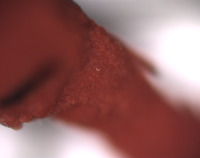
\includegraphics[width=0.5in, height=0.5in]{https://raw.githubusercontent.com/harkanatta/nfr21/main/myndir/1.jpg} & \cellcolor[HTML]{0D0887}{\textcolor{white}{\underline{Samsett litróf*}}} & \cellcolor[HTML]{0D0887}{\textcolor{white}{68.39}} & \cellcolor[HTML]{B32C8E}{\textcolor{white}{Polyvinyl Chloride 2}} & \cellcolor[HTML]{B32C8E}{\textcolor{white}{51.91}} & \cellcolor[HTML]{9511A1}{\textcolor{white}{Dyed Cellulose 4}} & \cellcolor[HTML]{9511A1}{\textcolor{white}{48.35}}\\

\includegraphics[width=0.5in, height=0.5in]{https://raw.githubusercontent.com/harkanatta/nfr21/main/myndir/10.jpg} & \cellcolor[HTML]{E26660}{\textcolor{white}{\underline{Loxiol HOB}}} & \cellcolor[HTML]{E26660}{\textcolor{white}{81.53}} & \cellcolor[HTML]{FAD824}{\textcolor{white}{Polyethylene 25}} & \cellcolor[HTML]{FAD824}{\textcolor{white}{91.64}} & \cellcolor[HTML]{ED7A52}{\textcolor{white}{Polyethylene 23}} & \cellcolor[HTML]{ED7A52}{\textcolor{white}{73.81}}\\
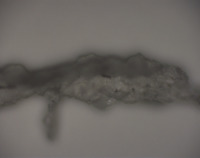
\includegraphics[width=0.5in, height=0.5in]{https://raw.githubusercontent.com/harkanatta/nfr21/main/myndir/11.jpg} & \cellcolor[HTML]{BBBBBB}{\textcolor{white}{\underline{}}} & \cellcolor[HTML]{BBBBBB}{\textcolor{white}{NA}} & \cellcolor[HTML]{0D0887}{\textcolor{white}{Polyethylene Terephthalate 14}} & \cellcolor[HTML]{0D0887}{\textcolor{white}{20.39}} & \cellcolor[HTML]{0D0887}{\textcolor{white}{Polyurethane 6}} & \cellcolor[HTML]{0D0887}{\textcolor{white}{25.86}}\\
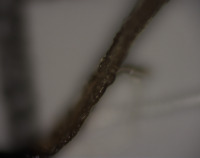
\includegraphics[width=0.5in, height=0.5in]{https://raw.githubusercontent.com/harkanatta/nfr21/main/myndir/12.jpg} & \cellcolor[HTML]{BBBBBB}{\textcolor{white}{\underline{}}} & \cellcolor[HTML]{BBBBBB}{\textcolor{white}{NA}} & \cellcolor[HTML]{F9973F}{\textcolor{white}{Polypropylene 10}} & \cellcolor[HTML]{F9973F}{\textcolor{white}{78.83}} & \cellcolor[HTML]{F68F44}{\textcolor{white}{Polypropylene 10}} & \cellcolor[HTML]{F68F44}{\textcolor{white}{78.14}}\\
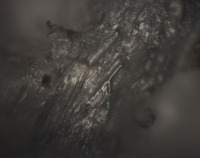
\includegraphics[width=0.5in, height=0.5in]{https://raw.githubusercontent.com/harkanatta/nfr21/main/myndir/13.jpg} & \cellcolor[HTML]{F0F921}{\textcolor{white}{\underline{Rutile}}} & \cellcolor[HTML]{F0F921}{\textcolor{white}{89.96}} & \cellcolor[HTML]{F8E125}{\textcolor{white}{Polypropylene 5}} & \cellcolor[HTML]{F8E125}{\textcolor{white}{93.27}} & \cellcolor[HTML]{F5EB27}{\textcolor{white}{Polypropylene 16}} & \cellcolor[HTML]{F5EB27}{\textcolor{white}{94.94}}\\
\addlinespace
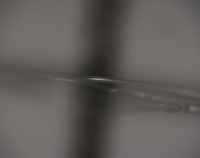
\includegraphics[width=0.5in, height=0.5in]{https://raw.githubusercontent.com/harkanatta/nfr21/main/myndir/14.jpg} & \cellcolor[HTML]{3F049C}{\textcolor{white}{\underline{Samsett litróf**}}} & \cellcolor[HTML]{3F049C}{\textcolor{white}{70.42}} & \cellcolor[HTML]{FCA835}{\textcolor{white}{Polyethylene 19}} & \cellcolor[HTML]{FCA835}{\textcolor{white}{82.34}} & \cellcolor[HTML]{FCA934}{\textcolor{white}{Polyethylene 25}} & \cellcolor[HTML]{FCA934}{\textcolor{white}{83.53}}\\
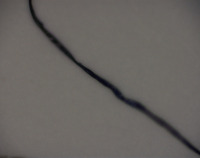
\includegraphics[width=0.5in, height=0.5in]{https://raw.githubusercontent.com/harkanatta/nfr21/main/myndir/15.jpg} & \cellcolor[HTML]{BBBBBB}{\textcolor{white}{\underline{}}} & \cellcolor[HTML]{BBBBBB}{\textcolor{white}{NA}} & \cellcolor[HTML]{8A09A5}{\textcolor{white}{Polyurethane 7}} & \cellcolor[HTML]{8A09A5}{\textcolor{white}{42.08}} & \cellcolor[HTML]{8104A7}{\textcolor{white}{Polystyrene-co-Polyvinyl Chloride 1}} & \cellcolor[HTML]{8104A7}{\textcolor{white}{44.26}}\\
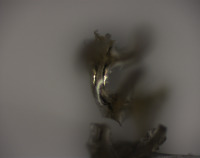
\includegraphics[width=0.5in, height=0.5in]{https://raw.githubusercontent.com/harkanatta/nfr21/main/myndir/16.jpg} & \cellcolor[HTML]{BBBBBB}{\textcolor{white}{\underline{}}} & \cellcolor[HTML]{BBBBBB}{\textcolor{white}{NA}} & \cellcolor[HTML]{5B01A5}{\textcolor{white}{Polyvinyl Chloride 6}} & \cellcolor[HTML]{5B01A5}{\textcolor{white}{32.89}} & \cellcolor[HTML]{5302A3}{\textcolor{white}{Polystyrene 3}} & \cellcolor[HTML]{5302A3}{\textcolor{white}{35.84}}\\
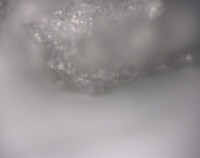
\includegraphics[width=0.5in, height=0.5in]{https://raw.githubusercontent.com/harkanatta/nfr21/main/myndir/2.jpg} & \cellcolor[HTML]{EB7655}{\textcolor{white}{\underline{Polyethylene}}} & \cellcolor[HTML]{EB7655}{\textcolor{white}{82.62}} & \cellcolor[HTML]{F0F921}{\textcolor{white}{Polyethylene 26}} & \cellcolor[HTML]{F0F921}{\textcolor{white}{97.50}} & \cellcolor[HTML]{F0F921}{\textcolor{white}{Polyethylene 16}} & \cellcolor[HTML]{F0F921}{\textcolor{white}{97.20}}\\
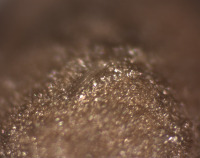
\includegraphics[width=0.5in, height=0.5in]{https://raw.githubusercontent.com/harkanatta/nfr21/main/myndir/3.jpg} & \cellcolor[HTML]{F89540}{\textcolor{white}{\underline{Samsett litróf***}}} & \cellcolor[HTML]{F89540}{\textcolor{white}{84.64}} & \cellcolor[HTML]{FEBE2A}{\textcolor{white}{Polyester 3}} & \cellcolor[HTML]{FEBE2A}{\textcolor{white}{86.87}} & \cellcolor[HTML]{FDB42F}{\textcolor{white}{Polyester 1}} & \cellcolor[HTML]{FDB42F}{\textcolor{white}{85.45}}\\
\addlinespace
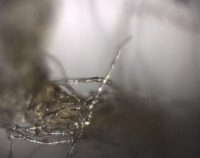
\includegraphics[width=0.5in, height=0.5in]{https://raw.githubusercontent.com/harkanatta/nfr21/main/myndir/4.jpg} & \cellcolor[HTML]{6E00A8}{\textcolor{white}{\underline{Samsett litróf****}}} & \cellcolor[HTML]{6E00A8}{\textcolor{white}{72.86}} & \cellcolor[HTML]{AD2793}{\textcolor{white}{Polypropylene 10}} & \cellcolor[HTML]{AD2793}{\textcolor{white}{50.47}} & \cellcolor[HTML]{A51F99}{\textcolor{white}{Polypropylene 10}} & \cellcolor[HTML]{A51F99}{\textcolor{white}{51.48}}\\
\bottomrule
\multicolumn{7}{l}{\rule{0pt}{1em}\textit{Note: }}\\
\multicolumn{7}{l}{\rule{0pt}{1em}Here is a general comments of the table. }\\
\multicolumn{7}{l}{\rule{0pt}{1em}\textsuperscript{1} Footnote 1; }\\
\multicolumn{7}{l}{\rule{0pt}{1em}\textsuperscript{2} Footnote 2; }\\
\multicolumn{7}{l}{\rule{0pt}{1em}\textsuperscript{3} rass}\\
\multicolumn{7}{l}{\rule{0pt}{1em}\textsuperscript{4} ress}\\
\end{tabular}
\end{table}

\end{document}
